\renewcommand*{\arraystretch}{1.1}

\subsection*{BI / read / 22}
\label{section:bi-read-22}

\noindent\begin{tabularx}{\queryCardWidth}{|>{\queryPropertyCell}p{\queryPropertyCellWidth}|X|}
	\hline
	query & BI / read / 22 \\ \hline
%
	title & International dialog
 \\ \hline
%
	pattern & \hfill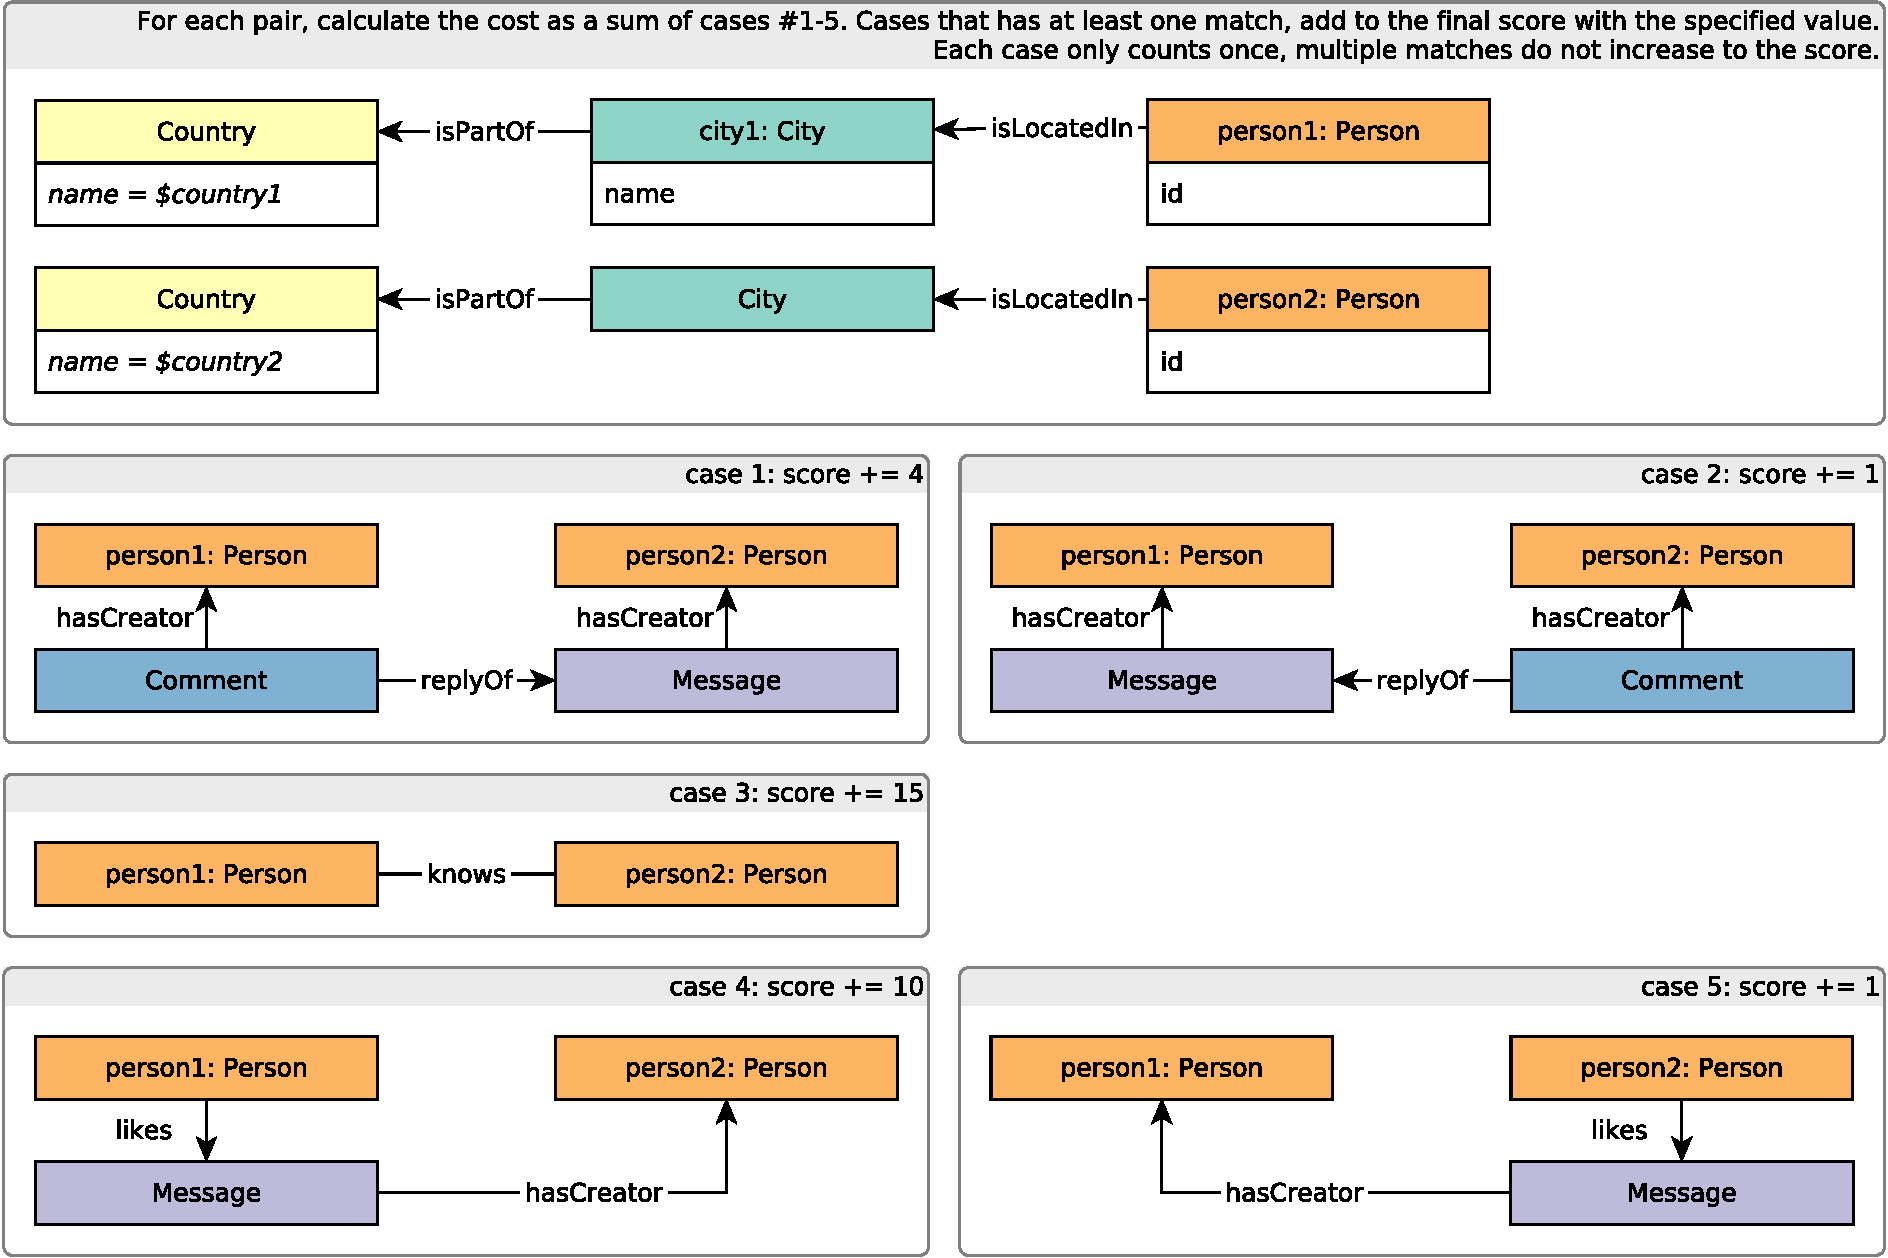
\includegraphics[scale=\patternscale,margin=0cm .2cm]{patterns/bi-read-22}\hfill\vadjust{} \\ \hline
%
	desc. & Consider all pairs of people \texttt{(p1,\ p2)} such that one is located
in a city of Country \texttt{countryX} and the other is located in a
city of Country \texttt{countryY}.

For each city of Country \texttt{countryX}, return the highest scoring
pair.

The score of a pair is defined as the sum of the scores of the following
kinds of interaction:

\begin{itemize}
\tightlist
\item
  \texttt{p1} has created a reply Comment to at least one Comment or
  Post by \texttt{p2}: \texttt{Score\ =\ 4}
\item
  \texttt{p1} has created at least one Post or Comment that \texttt{p2}
  has created a reply Comment to: \texttt{Score\ =\ 1}
\item
  \texttt{p1} and \texttt{p2} Know each other: \texttt{Score\ =\ 15}
\item
  \texttt{p1} liked at least one Post or Comment by \texttt{p2}:
  \texttt{Score\ =\ 10}
\item
  \texttt{p1} has created at least one Post or Comment that was liked by
  \texttt{p2}: \texttt{Score\ =\ 1}
\end{itemize}

Consequently, the maximum score a pair can obtain is:
\texttt{4\ +\ 1\ +\ 15\ +\ 10\ +\ 1\ =\ 31}
 \\ \hline
%
	
		params &
		\innerCardVSpace{\begin{tabularx}{\attributeCardWidth}{|>{\paramNumberCell}c|>{\varNameCell}M|>{\typeCell}m{\typeWidth}|Y|} \hline
		$\mathsf{1}$ & countryX
 & String
 &  \\ \hline
		$\mathsf{2}$ & countryY
 & String
 &  \\ \hline
		\end{tabularx}}\innerCardVSpace \\ \hline
	
%
	
		result &
		\innerCardVSpace{\begin{tabularx}{\attributeCardWidth}{|>{\resultNumberCell}c|>{\varNameCell}M|>{\typeCell}m{\typeWidth}|>{\resultOriginCell}c|Y|} \hline
		$\mathsf{1}$ & p1.id
 & 64-bit Integer
 & R &
				 \\ \hline
		$\mathsf{2}$ & p2.id
 & 64-bit Integer
 & R &
				 \\ \hline
		$\mathsf{3}$ & cityX.name
 & String
 & R &
				 \\ \hline
		$\mathsf{4}$ & score
 & 32-bit Integer
 & R &
				 \\ \hline
		\end{tabularx}}\innerCardVSpace \\ \hline
	
%
	
		sort		&
		\innerCardVSpace{\begin{tabular}{|>{\sortNumberCell}c|>{\varNameCell}l|>{\directionCell}c|} \hline
		$\mathsf{1}$ & score
 & $\desc
$ \\ \hline
		$\mathsf{2}$ & p1.id
 & $\asc
$ \\ \hline
		$\mathsf{3}$ & p2.id
 & $\asc
$ \\ \hline
		\end{tabular}}\innerCardVSpace \\ \hline
	%
	%
	CPs &
	\multicolumn{1}{>{\raggedright}l|}{
		\chokePoint{1.4}, 
		\chokePoint{1.6}, 
		\chokePoint{2.1}, 
		\chokePoint{3.1}, 
		\chokePoint{3.3}, 
		\chokePoint{5.1}, 
		\chokePoint{5.2}, 
		\chokePoint{5.3}
		} \\ \hline
	%
	%
\end{tabularx}
\queryCardVSpace